% nezavisnost definicije

\chapter{Definicije}

U ovom cijelom poglavlju $\vjerojatnosniProstor$ je vjerojatnosni prostor.
Doga\dj aji $A, \; B \in \famF$ su nezavisni ako vrijedi:
\begin{equation*}
    \vjeroj{A \cap B} = \vjeroj{A} \cdot \vjeroj{B}.
\end{equation*}

\begin{pr}  \label{pr:6.1}
    Iako se nezavisnost jako \v cesto primjenjuje, zapravo se "rijetko" doga\dj a
    % slika
    \begin{figure}[H]
        \centering
        \begin{subfigure}[b]{0.45\textwidth}
            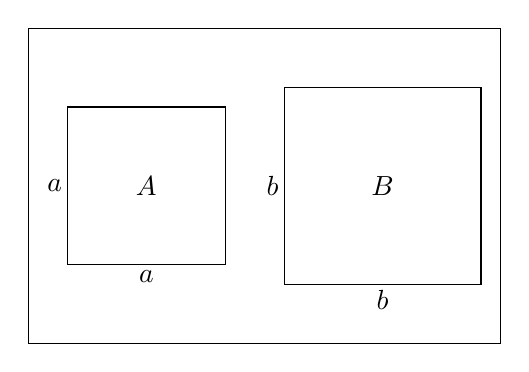
\begin{tikzpicture}
                \draw (0, 0) rectangle (6, 4);
                \draw (0.5, 1) rectangle (2.5, 3);
                \draw (3.25, 0.75) rectangle (5.75, 3.25);
                \node at (0.5, 2) [label=left:$a$, xshift=5pt] {};
                \node at (1.5, 1) [label=below:$a$, yshift=5pt] {};
                \node at (4.5, 0.75) [label=below:$b$, yshift=5pt] {};
                \node at (3.25, 2) [label=left:$b$, xshift=5pt] {};
                \node at (1.5, 2) [label=center:$A$] {};
                \node at (4.5, 2) [label=center:$B$] {};
            \end{tikzpicture}
        \end{subfigure}
        %%%%%%%
        \begin{subfigure}[b]{0.45\textwidth}
            \begin{tikzpicture}
                \draw (0, 0) rectangle  (6, 4);
                \draw (1.25, 1) rectangle (3.25, 3);
                \draw (2.75, 0.75) rectangle (5.25, 3.25);
                \fill[pattern=south west lines] (2.75, 1) rectangle (3.25, 3);
                \node at (1.25, 2) [label=left:$a$, xshift=5pt] {};
                \node at (2.25, 1) [label=below:$a$, yshift=5pt] {};
                \node at (4, 0.75) [label=below:$b$, yshift=5pt] {};
                \node at (5.25, 2) [label=right:$b$, xshift=-5pt] {};
                \node at (2.25, 2) [label=center:$A$] {};
                \node at (4, 2) [label=center:$B$] {};
                \node at (3, 1) [label=above:$x$, yshift=-5pt] {};
            \end{tikzpicture}
        \end{subfigure}
    \end{figure}
    \begin{equation*}
        \begin{aligned}
            \vjeroj{A} &= a^2\\
            \vjeroj{B} &= b^2\\
            \vjeroj{A \cap B} &= a \cdot x
        \end{aligned}
    \end{equation*}
    Odakle vidimo da slijedi:
    \begin{equation*}
        \vjeroj{A \cap B} = \vjeroj{A} \cdot \vjeroj{B} \iff x = a b^2.
    \end{equation*}
\end{pr}

Lako se vidi:\\
%$A$ je nezavisan sam sa sobom ako i samo ako je $\vjeroj{A} = 0 \lor %\vjeroj{A} = 1$ ako i samo ako $A$ i $B$ su nezavisni za svaki $B \in \famF$.
\begin{align}   \label{jed:6.2}
    \begin{split}
        \begin{matrix}
            A \textnormal{ je nezavisan}\\
            \textnormal{sa samim sobom}
        \end{matrix}
        &\iff
        \vjeroj{A} \in \{0, \; 1\}\\
        &\iff
        \begin{matrix}
            \textnormal{$A$ i $B$ su nezavisni}\\
            \textnormal{za svaki } B \in \famF
        \end{matrix}
    \end{split}
\end{align}

Laki ra\v cun tipa
\begin{align*}
    \vjeroj{A \cap B^c} &= 1 - \vjeroj{A^c \cup B} = 1 - \vjeroj{A^c \cup (A \cap B)}\\
    &= 1 - \vjeroj{A^c} - \vjeroj{A \cap B} = (\textnormal{nezavisnost})\\
    &= \vjeroj{A} - \vjeroj{A} \cdot \vjeroj{B}\\
    &= \vjeroj{A} \cdot \vjeroj{B^c}
\end{align*}
daje:
\begin{align}   \label{jed:6.3}
    \begin{split}
        A, \; B \textnormal{ nezavisni} &\iff A, \; B^c \textnormal{ nezavisni}\\
        &\iff A^c, \; B \textnormal{ nezavisni}\\
        &\iff A^c, \; B^c \textnormal{ nezavisni}.
    \end{split}
\end{align}

\v Sto ako imamo 3 ili vi\v se doga\dj aja?
Treba biti oprezan.
Doga\dj aji $A_1, \ldots, A_n \in \famF$ su nezavisni ako za svaki $k \in \{1, \ldots, n\}$ i svaki izbor me\dj usobno razli\v citih $i_1, \ldots, i_k \in \{1, \ldots, n\}$ vrijedi $\vjeroj{A_{i_1} \cap \ldots  \cap A_{i_k}} = \vjeroj{A_{i_1}} \cdot \ldots \cdot \vjeroj{A_{i_k}}$.

\begin{zad} \label{zad:6.4}
    Na\dj ite primjere tri doga\dj aja $A, \: B, \: C \in \famF$ koji nisu nezavisni, ali za njih vrijedi:
    \begin{enumerate}[label=(\roman*)]
        \item U praovima su nezavisni
        \item $\vjeroj{A \cap B \cap C} = \vjeroj{A} \: \vjeroj{B} \: \vjeroj{C}$.
    \end{enumerate}
\end{zad}

\begin{zad} \label{zad:6.5}
    Doka\v zite da dodavanjem ili oduzimanjem doga\dj aja vjerojatnosti $0$ ili $1$, ne\' cemo promjeniti "status" nezavisnosti kona\v cne familije doga\dj aja.
\end{zad}

Je li uvijek jednostavno "intuitivno" prepoznati nezavisnost?

\begin{pr}  \label{pr:6.6}
    Promatramo obitelj s troje djece i pretpostavljamo da su svih 8 mogu\' cnosti (\v z\v z\v z, \v z\v zm, ..., mmm) jednako vjerojatne.
    Lako se vidi da su $A =$ "postoje oba spola" i $B = $ "postoji najvi\v se jedno \v zensko djete" nezavisni ($\vjeroj{A} = \frac{6}{8}, \; \vjeroj{B} = \frac{4}{8}, \; \vjeroj{A \cap B} = \frac{3}{8}$).
    \v Sto ako iste doga\dj aje promatramo za obitelji s 4 djece? Tada vi\v se nisu.
\end{pr}

Vrijedi li ne\v sto poput \eqref{jed:6.3} za slu\v caj $n$ doga\dj aja?
Zapravo da. Nije te\v sko za pokazati:
\begin{equation}    \label{jed:6.7}
    \begin{matrix}
        A_1, \ldots, A_n \in \famF\\
        \textnormal{su nezavisni doga\dj aji}
    \end{matrix}
    \iff
    \begin{matrix}
        \textnormal{za svaki od $2^n$ izbora doga\dj aja}\\
        B_1 \in \{A_1, \: A_1^c\}, \ldots, B_1 \in \{A_n, \: A_n^c\}\\
        \vjeroj{B_1 \cap \ldots \cap B_n} = \vjeroj{B_1} \: \ldots \: \vjeroj{B_n}
    \end{matrix}
    .
\end{equation}

Uo\v cimo da \eqref{jed:6.3} i \eqref{jed:6.7} navode na to da su nezavisnosti doga\dj aja zapravo posebni slu\v cajevi nezavisnosti familija doga\dj aja.

\begin{defn}    \label{defn:6.8}
    Neka je $\Lambda \neq \varnothing$ i $\indFamilija{\famG_\lambda}{\lambda \in \Lambda}$ indeksirani skup familija doga\dj aja, to jest $\famG_\lambda \subseteq \famF, \; \forall \lambda \in \Lambda$.
    Tada je $\indFamilija{\famG_\lambda}{\lambda \in \Lambda}$ \emph{nezavisna} (ili nepreciznije, \emph{familije} $\famG_\lambda$ \emph{su me\dj usobno nezavisne}), ako, za svaki $n \in \nat \setminus \{1\}$, za svaki izbor me\dj usobno razli\v citih $\lambda_1, \ldots, \lambda_n \in \Lambda$ i za svaki izbor $A_1 \in \famG_{\lambda_1}, \ldots, A_n \in \famG_{\lambda_n}$, vrijedi:
    \begin{equation*}
        \vjeroj{A_1 \cap \ldots \cap A_n} = \vjeroj{A_1} \cdot \ldots \cdot \vjeroj{A_n}.
    \end{equation*}
\end{defn}

\begin{nap} \label{nap:6.9}
    \begin{enumerate}[label=(\alph*)]
        \item Od posebnog interesa je slu\v caj kada su sve $\famG_{\lambda_n}$ $\sigma$-algebre.
        \item $A, \; B$ su nezavisni $\iff$ $\{A\}, \; \{B\}$ nezavisne $\iff$ $\sigma$-algebre $\{ \varnothing, \: A, \: A^c, \: \Omega \}$, $\{ \varnothing, \: B, \: B^c, \: \Omega \}$ nezavisne.
        \item   \label{nap:6.9c}
        Sada se mo\v ze tretirati proizvoljna familija doga\dj aja.
        Ako je $\indFamilija{A_t}{t \in T} \subseteq \famF$, tada su $A_t, t \in T$, me\dj usuobno nezavisne ako su familije $\{A_t\}, \; t \in T$, me\dj usobno nezavisne.
        Lako se vidi da je to ispunjeno ako i samo ako je svaka kona\v can potfamilija na\v se familije sastavljena od me\dj usobno nezavisnih doga\dj aja.
        \item \label{nap:6.9d}
        Ako (u definiciji \ref{defn:6.8}) imamo $\famH_\lambda \subseteq \famG_\lambda, \; \forall \lambda \in \Lambda$, tada nezavisnost familija $\famG_\lambda, \; \lambda \in \Lambda$, implicira nezavisnost familija $\famH_\lambda, \; \lambda \in \Lambda$ (dokaz je trivijalan).
        \item Ako (u definiciji \ref{defn:6.8}) imamo $\tilde{\Lambda} \subseteq \Lambda$ i $\tilde{\Lambda} \neq \varnothing$, tada nezavisnost familija $\famG_\lambda, \; \lambda \in \Lambda$, implicira nezavisnost familija $\famG_\lambda, \; \lambda \in \tilde{\Lambda}$.
        \item \label{nap:6.9f}
        Uo\v cimo da definicija \ref{defn:6.8} uklju\v cuje i slu\v caj kada je neka od $\famG_\lambda = \varnothing$.
        Dodavanje ili oduzimanje takve familije unutar indeksiranog skupa $\{\famG_\lambda\}$ ne mjenja "status nezavisnosti" istog.
        Ako gledamo nadklase takvih $\famG_\lambda$, onda obi\v cno koristimo konvenciju $\sigAlg{\varnothing} = \{ \varnothing, \; \Omega\}$.
    \end{enumerate}
\end{nap}

O\' cito, smanjivati klase na razne na\v cine ne\' ce ugroziti nezavisnost.
\v Sto ako pove\' camo?

\begin{tm}  \label{tm:6.10}
    Neka je $\Lambda \neq \varnothing$ i $\indFamilija{\famG_\lambda}{\lambda \in \Lambda}$ indeksirani skup $\pi$-sistema doga\dj aja, to jest $\famG_\lambda \subseteq \famF$, za svaki $\lambda \in \Lambda$ i $\famG_\lambda$ je $\pi$-sistem, za svaki $\lambda \in \Lambda$.
    Ako je $\indFamilija{\famG_\lambda}{\lambda \in \Lambda}$ nezavisna, tada je i $\indFamilija{\sigAlg{\famG_\lambda}}{\lambda \in \Lambda}$ nezavisna.
\end{tm}

\begin{proof}
    Bez smanjenja op\' cenitosti, vidi napomenu \ref{nap:6.9} \ref{nap:6.9f}, uzmimo $\famG_\lambda \neq \varnothing$, za svaki $\lambda \in \Lambda$.
    Neka je $n \geq 2$, $\lambda_1, \ldots, \lambda_n \in \Lambda$, me\dj usobno razli\v citi i fiksirajmo izbor $A_1 \in \famG_{\lambda_1}, \ldots, A_n \in \famG_{\lambda_n}$.
    Promatramo familiju:
    \begin{equation*}
        \famD_1 := \skup{B \in \famF}{\vjeroj{B \cap A_2 \cap \ldots \cap A_n} = \vjeroj{B} \: \vjeroj{A_2} \ldots \vjeroj{A_n}}.
    \end{equation*}
    Po pretpostavci je $\famG_{\lambda_1} \subseteq \famD_1$.
    O\v cito je i $\Omega \in \famD_1$.
    Ako su $B_1, \; B_2 \in \famD_1$ i $B_1 \subseteq B_2$, tada vrijedi
    \begin{align*}
        \vjeroj{(B_2 \setminus B_1) \cap A_2 \cap \ldots \cap A_n} &= \vjeroj{B_2 \cap A_2 \cap \ldots \cap A_n} - \vjeroj{B_1 \cap A_2 \cap \ldots \cap A_n} \\
        &= [\vjeroj{B_2} - \vjeroj{B_1}] \: \vjeroj{A_2} \ldots \vjeroj{A_n}\\
        &= \vjeroj{B_2 \setminus B_1} \: \vjeroj{A_2} \ldots \vjeroj{A_n},
    \end{align*}
    odakle vidimo da je $B_2 \setminus B_1 \in \famD_1$.
    Sli\v cno dobijemo i
    \begin{equation*}
        \niz{B_n}{n \in \nat} \subseteq \famD_1, \quad B_n \nearrow B \implies B \in \famD_1.
    \end{equation*}
    Slijedi da je $\famD_1$ Dynkinova klasa koja sadr\v zi $\pi$-sistem $\famG_{\lambda_1}$.
    Stoga $\sigAlg{\famG_{\lambda_1}} \subseteq \famD_1$.
    Neka je sada $C_1 \in \sigAlg{\famG_{\lambda_1}}$ proizvoljan i:
    \begin{equation*}
        \famD_2 := \skup{B \in \famF}{\vjeroj{C_1 \cap B \cap A_3 \cap \ldots \cap A_n} = \vjeroj{C_1} \: \vjeroj{B} \: \vjeroj{A_3} \ldots \vjeroj{A_n}}.
    \end{equation*}
    Kako je $A_2 \in \famG_{\lambda_2}$ bio proizvoljan, slijedi da je $\famG_{\lambda_2} \subseteq \famD_2$, a lako se poka\v ze da je $\famD_2$ Dynkinova klasa.
    Slijedi $\sigAlg{\famG_{\lambda_2}} \subseteq \famD_2$.
    Time smo pokazali da za svaki izbor $B_1 \in \sigAlg{\famG_{\lambda_1}}, \; B_2 \in \sigAlg{\famG_{\lambda_2}}, \: A_3 \in \famG_{\lambda_3} \ldots, A_n \in \famG_{\lambda_n}$ vrijedi:
    \begin{equation*}
        \vjeroj{B_1 \cap B_2 \cap A_3 \cap \ldots \cap A_n} = \vjeroj{B_1} \: \vjeroj{B_2} \: \vjeroj{A_3} \ldots \vjeroj{A_n}.
    \end{equation*}
    Sada je jasno kako induktivno nastavoljamo s ovim dokazom i nakon kona\v cno mnogo koraka dobijemo \v zeljenu tvrdnju.
\end{proof}

\begin{kor} \label{kor:6.11}
    Neka je $\Lambda \neq \varnothing, \: \famF_\lambda \subseteq \famF$ $\sigma$-algebra za svaki $\lambda \in \Lambda$ i $\indFamilija{\famF_\lambda}{\lambda \in \Lambda}$ nezavisna.
    Ako je $\famT$ particija skupa $\Lambda$ i za svaki $T \in \famT$,
    \begin{equation*}
        \famF_T := \indSigAlg{\famF_\lambda}{\lambda \in T},
    \end{equation*}
    tada je $\indFamilija{\famF_T}{T \in \famT}$ nezavisna.
\end{kor}

\begin{nap}
    Prethodni korolar govori da disjunktni komadi ostaju nezavisni.
    \begin{equation*}
        \underbrace{\famF_{\lambda_1}, \ldots, \famF_{\lambda_n}} , \underbrace{\famF_{\lambda_{n + 1}}, \ldots}, \ldots
    \end{equation*}
\end{nap}

\begin{proof}
    Za $T \in \famT$ difiniramo $\pi$-sistem
    \begin{equation*}
        \famG_T := \indFamilija{A_1 \cap \ldots \cap A_n}{n \in \nat, \; A_i \in \unija{\lambda \in T}{}\famF_\lambda}.
    \end{equation*}
    Budu\' ci da su $\famF_\lambda$ $\sigma$-algebre, slijedi
    \begin{align*}
        \famG_T := \{B_1 \cap \ldots \cap B_n \: | \: &n \in \nat, \; n \leq \card{T}, \; \lambda_1, \ldots, \lambda_n \in T \textnormal{ me\dj usobno razli\v citih},\\ &B_1 \in \famF_{\lambda_1},\ldots, B_n \in \famF_{\lambda_n}\},
    \end{align*}
    \v sto daje da su $\indFamilija{\famG_T}{T \in \famT}$ nezavisne.
    Sada tvrdnja slijedi iz teorema \ref{tm:6.10} i $\sigAlg{\famG_T} = \famF_T$.
\end{proof}

\begin{prop}    \label{prop:6.12}
    Neka je $\Lambda \neq \varnothing$, $\famF_\lambda \subseteq \famF$ $\sigma$-algebra za svaki $\lambda \in \Lambda$.
    Neka je $\famT \subseteq \partitive{\Lambda}$ separiraju\' ca klasa na $\Lambda$ (to jest za svaki $\mu, \; \lambda \in \Lambda, \; \lambda \neq \mu$, postoji $T \in \famT$ takav da $\card{T \cap \{\lambda, \; \mu\}} = 1$).
    Tada je $\indFamilija{\famF_\lambda}{\lambda \in \Lambda}$, nezavisna ako i samo ako je, za svako $T \in \famT$,
    \begin{equation*}
        \{ \indSigAlg{\famT}{t \in T}, \; \indSigAlg{\famF_t}{t \in T^c} \},
    \end{equation*}
    nezavisna.
\end{prop}

\begin{proof}
    \begin{enumerate}
        \item[$\implies$] Prema korolaru \ref{kor:6.11}.
        \item[$\impliedby$] Uo\v cimo da je dovoljno pokazati da za svaki kona\v can skup $S \subseteq \Lambda$ vrijedi $\indFamilija{\famF_\lambda}{\lambda \in S}$ nezavisna.
        Dokaz provodimo indukcijom po $\card{S}$.
        Za $\card{S} = 1$ tvrdnja trivijalno vrijedi.
        Pretpostavljamo da vrijedi za $\card{S} \leq n$ i uz tu pretpostavku promatramo skup $V \subseteq \Lambda$, $\card{V} = n + 1$.
        Posebno, $V$ sadr\v zi barem dva razli\v cita elementa iz $\Lambda$, recimo $\lambda$ i $\mu$, pa postoji $T \in \famT$ koji ih razlikuje.
        Posebno $V \cap T$ i $V \setminus T$ su neprazni skupovi.
        Po pretpostavci su $\indSigAlg{\famF_t}{t \in T}$ i $\indSigAlg{\famT}{t \in T^c}$ nezavisne, pa prema napomeni \ref{nap:6.9}  \ref{nap:6.9d} su $\indSigAlg{\famF_t}{t \in V \cap T}$ i $\indSigAlg{\famF_t}{t \in V \setminus T}$ nezavisne.
        Tada je $\presjek{\lambda \in V}{} A_\lambda = B \cap C$, pri \v cemu je $B = \presjek{\lambda \in V \cap T}{} A_\lambda$, $C = \presjek{\lambda \in V \setminus T}{} A_\lambda$.
        Tada je $\vjeroj{B \cap C} = \vjeroj{B} \: \vjeroj{C}$, a $\card{V \cap T} \leq n$ i $\card{V \setminus T} \leq n$.
        Po pretpostavci indukcije dobivamo
        \begin{equation*}
            \vjeroj{\presjek{\lambda \in V}{} A_\lambda} = \produkt{\lambda \in V}{} \vjeroj{A_\lambda}.
        \end{equation*}
    \end{enumerate}
\end{proof}

\begin{zad} \label{zad:6.13}
    Neka je $\famF_n \subseteq \famF$ $\sigma$-algebra, za svaki $n \in \nat$.
    Ako su, za svaki $n \in \nat$, nezavisne $\sigma$-algebre $\indSigAlg{\famF_k}{k \leq n}$ i $\famF_{n + 1}$, je li tada i $\indFamilija{\famF_n}{n \in \nat}$ nezavisna?
    \v Sto ako pretpostavimo da su $\famF_m$ i $\famF_n$ nezavisne, \v cim su $n, \; m \in \nat$ i $n \neq m$?
\end{zad}

\begin{zad} \label{zad:6.14}
    Neka je $\indFamilija{A_n}{n \in \nat} \subseteq \famF$ familija nezavisnih doga\dj aja.
    Vrijedi li
    \begin{equation*}
        \vjeroj{\presjek{n \in \nat}{} A_n} = \produkt{n \in \nat}{} \vjeroj{A_n}?
    \end{equation*}
\end{zad}